\section{Stromsteuerkennlinie}
\subsection{Experimentelle Durchf\"urung}
In diesem Versuch wird die Stromsteuerkennlinie I$_C$ $=$ f(I$_B$) des NPN-Transistors BC 547C aufgenommen. Aus dieser Kennlinie wird anschlie\ss end die Gro\ss signalstromverst\"arkung B sowie die Kleinsignalstromverst\"arkung $\beta$ f\"ur verschiedene Arbeitspunkte ermittelt.
\begin{figure}[!h]
\begin{center}
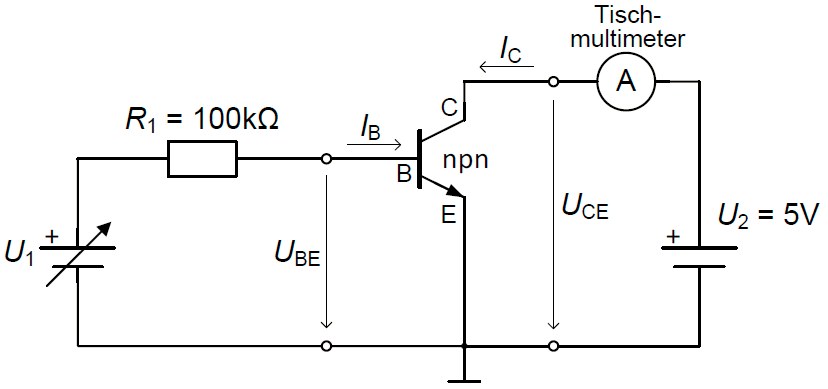
\includegraphics[width=0.8\textwidth]{stromSteuerKennlinie}
\caption{Der Versuchsaufbau zur Bestimmung der Stromsteuerkennlinie des Transistors}
\end{center}
\end{figure}
\newpage
\subsection{Ergebnisse und Diskussion}
In Tabelle 2 sind die Ergebnisse der Messung und der Simulation des Kollektorstroms I$_C$ in Abh\"angigkeit des Basisstroms I$_B$ bestimmt.
\begin{figure}[!h]
\begin{center}
\textbf{Tabelle 2: Aufgenommene Messwerte von I$_{C}$ in Abh\"angigkeit von I$_B$ f\"ur U$_2$ $=$ 5~$V$} \\[0.2cm]
%\caption{}
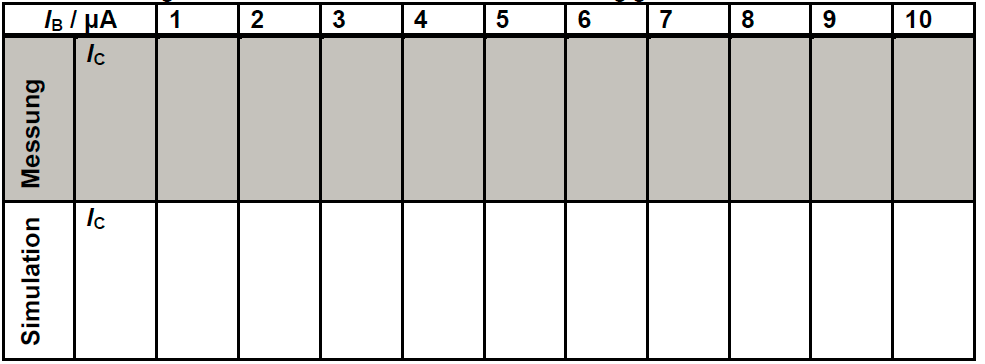
\includegraphics[width=0.8\textwidth]{ergebnissVersuch2}
\end{center}
\end{figure}
\vspace{10cm}
\begin{figure}[!h]
\begin{center}
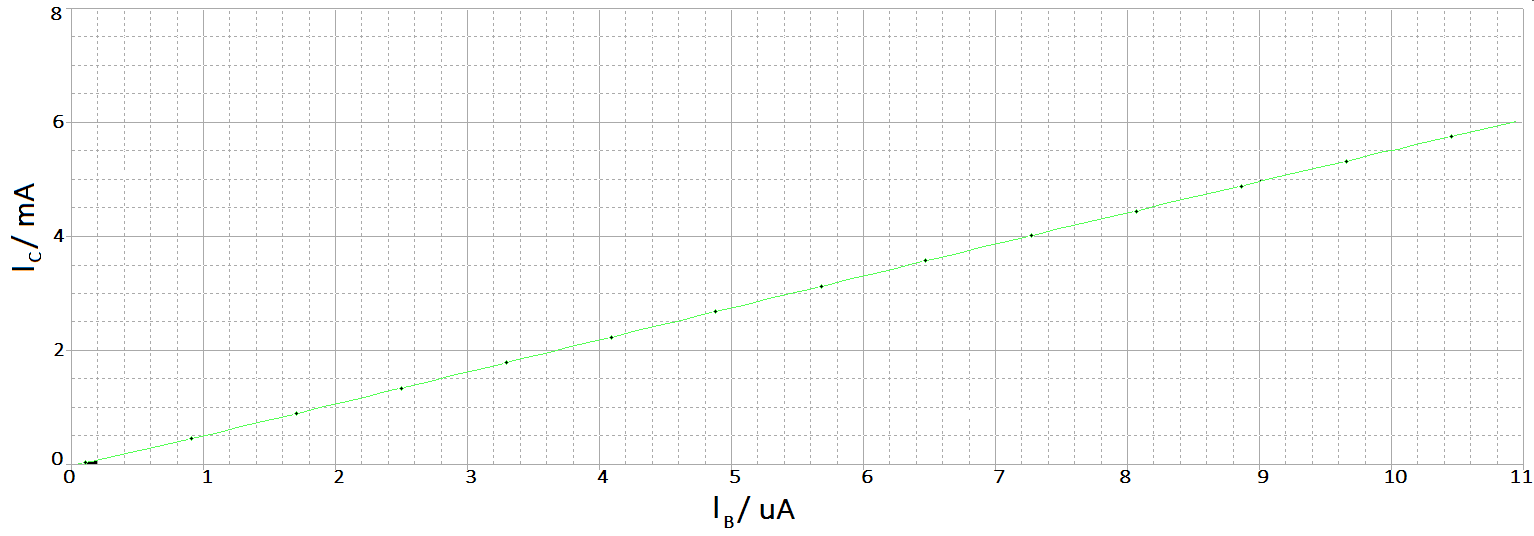
\includegraphics[width=1\textwidth]{Versuch2}
\caption{Graphische Darstellung der simulierten Ergebnisse}
\end{center}
Die Abbildung (4) zeigt einen linearen Anstieg des Kollektorstroms \"uber den Basisstrom. Eine charakteristische Gr\"o\ss e f\"ur einen bestimmten Transistor ist sein Stromverst\"arkungsfaktor \textbf{B}, also das Verh\"altnis, dass in Abbildung (3) angegeben ist. Genaugenomen ist die Stromverst\"arkung abh\"angig vom
Kollektorstrom und von der Kollektor-Emitterspannung, sodass sie nur f\"ur
einen bestimmten Arbeitspunkt bestimmt werden kann.
\end{figure}
\vspace{15cm}
\begin{equation}
\textbf{B} = \frac{\textbf{I$_C$}}{\textbf{I$_B$}}
\end{equation}
\begin{equation}
\textbf{$\beta$} = \frac{\textbf{$\Delta$I$_C$}}{\textbf{$\Delta$I$_B$}}
\end{equation}
Die Klein- bzw Gro\ss signalverst\"arkung lassen sich durch die Gleichungen (3) und (4) bestimmen, die Ergebnisse siehe Tabelle (mit I$_B$ $=$ 3~$\mu A$): \\
\begin{center}
\begin{tabular}{|l|l|l|}
\hline
Messreihe & Simulation & Messung \\
\hline 
\textbf{B} & & \\
\hline
$\beta$ & & \\
\hline
\end{tabular}
\end{center}
Es zeigt sich, dass die Kleinsignal- \textbf{$\beta$} bzw Gleichsignalstromverst\"arkung \textbf{B} sich sehr \"ahneln :\begin{equation*}
\beta \approx \text{\textbf{B}}
\end{equation*} 